\section{Usability Sicht}
Dieses Unterkapitel definiert den Begriff \enquote{Usability} (deutsch: Gebrauchstauglichkeit). Mit der Gebrauchstauglichkeit im Vordergrund und den speziellen Bedürfnissen der Patient/innen muss die Anwendung zusätzlich angepasst werden. Daher werden die speziellen Designentscheidungen zugunsten der Behandelten beschrieben. Zuletzt wird noch auf die nachträglichen Änderungen eingegangen, die aufgrund von Problemen vorgenommen werden mussten.

\subsection{Usability}
Unter \enquote{Usability} wird oft ein Qualitätsmerkmal für das Entwerfen einer Benutzeroberfläche subsummiert. Zu diesen Merkmalen zählen unter anderem die Anordnung von Bedienelementen, die Anzahl der Klicks um zum Ziel zu gelangen oder die Einfachheit der Anwendung. \cite{richter:2013:usability} \\ 
Der Begriff \enquote{Usability} besteht aus mehreren Komponenten und wird häufig mit diesen fünf Kriterien in Verbindung gebracht: \cite{nielsen:1993:usability}

\begin{itemize}
    \item \textbf{Erlernbarkeit}: Die Einarbeitungszeit der Benutzer/innen in die Anwendung sollte möglichst gering sein.
    \item \textbf{Effizienz}: Das System sollte nach der Einarbeitungsphase sofort nutzbar sein.
    \item \textbf{Einprägsamkeit}: Gelegenheitsbenutzer/innen sollten das System nach längerer Abstinenz problemlos bedienen können, ohne das alles neu gelernt werden muss.
    \item \textbf{Fehler}: Dem/Der Benutzer/in sollten möglichst wenige Fehler bei der Benutzung des Systems unterlaufen. Die gemachten Fehler sollten ohne Probleme korrigierbar sein.
    \item \textbf{Zufriedenheit}: Das System sollte angenehm zu verwenden sein, damit der/die Benutzer/in zufrieden ist.
\end{itemize}

\subsubsection{10 Prinzipien für Interaktions-Design}
\citeauthor{nielsen:1993:usability} hat 1993 10 Prinzipien für gutes Interaktions-Design veröffentlicht. In diesem Abschnitt wird nun näher auf die einzelnen Prinzipien eingegangen, sowie Beispiele zu allen Punkten genannt, die in Zusammenhang mit der entwickelten Applikation stehen.

\paragraph{Simple and natural dialogue}
Dialoge sollen nur Informationen enthalten, die relevant sind. Jede zusätzliche Information steht in Konkurrenz zu anderen und verringert deren Sichtbarkeit. Alle Informationen sollten in einer logischen Reihenfolge sein. \cite{nielsen:1993:usability}

Die Applikation zeigt immer nur eine Information gleichzeitig. Wenn mehrere Meldungen gleichzeitig angezeigt werden, könnte dies den/die Benutzer/in überfordern.

\paragraph{Speek the users' language}
Dialoge sollen in einfachen Worten, Phrasen und Konzepten ausgedrückt werden, die dem/der Benutzer/in bereits bekannt sind. Technische Begriffe, die die meisten Benutzer/innen nicht interpretieren können, sollen nicht verwendet werden. \cite{nielsen:1993:usability}

In Erfolgs- und Fehlermeldungen der Anwendung sind keinerlei technische Begriffe versteckt. Die Hilfetexte sind in natürlicher Sprache verfasst und bieten wenig Interpretationsspielraum.

\paragraph{Minimize the users' memory load}
Benutzer/innen sollen sich nicht unnötig viele Informationen über mehrere Systemschritte merken. Wichtige Hinweise müssen immer sichtbar oder aufrufbar sein. \cite{nielsen:1993:usability}

Jeder Abschnitt des Spiels ist unabhängig voneinander. Der/Die Benutzer/in muss sich außer dem Rezept keinerlei relevante Information merken. Statistiken können im Nachhinein einfach betrachtet werden.

\paragraph{Consistency}
Für den/die Benutzer/in ist es wichtig, dass gewisse Design-Standards eingehalten werden. Gewisse Standards im Design der Oberflächen helfen besser mit dem System zurechtzukommen. Zur Konsistenz gehört auch eine konsistente Benutzer/innenführung. Das bedeutet, dass immer gleiche Begriffe für gleiche Aktionen verwendet werden sollen. \cite{nielsen:1993:usability}

Die Anwendung verwendet ein durchgehend konsistentes Farbdesign. Gewisse Bedienelemente werden immer wieder verwendet, damit sich der/die Benutzer/in einfach zurecht findet.

\paragraph{Feedback}
Der/Die Benutzer/in soll über den aktuellen Systemzustand informiert werden. Direkt nach einer Aktion muss positives oder negatives Feedback zur Situation gegeben werden. \cite{nielsen:1993:usability}

Beispielsweise wird der/die Benutzer/in darauf hingewiesen, dass der jeweilige Spielabschnitt erfolgreich beendet wurde (siehe Abbildung \ref{fig:game-success-message}).

\begin{figure}[H]
    \centering
	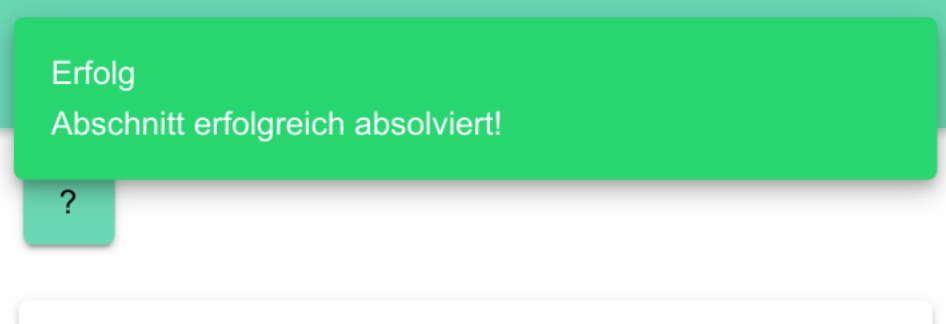
\includegraphics[width=0.5\linewidth]{figures/development/application/success-message.png}
	\caption{Erfolgsmeldung, die angezeigt wird, wenn der/die Spieler/in einen Abschnitt erfolgreich absolviert hat.}
	\label{fig:game-success-message}
\end{figure}

\paragraph{Clearly marked exits}
Benutzer/innen passieren immer wieder Fehler, wenn sie in der Applikation navigieren. Dabei soll es möglich sein, dass der/die User/in diesen ungewollten Zustand schnell verlassen kann, ohne dabei unnötig lange aufgehalten zu werden. \cite{nielsen:1993:usability}

Wenn ein/e Benutzer/in eine falsche Option anklickt, dann sollte diese/r nicht die komplette Aktion durchführen müssen, bevor fortgefahren wird. Das Spiel kann zu jeder Zeit abgebrochen werden, wenn es ungewollt gestartet wurde (siehe Abbildung \ref{fig:game-abort-page}).

\begin{figure}[H]
    \centering
    \frame{
	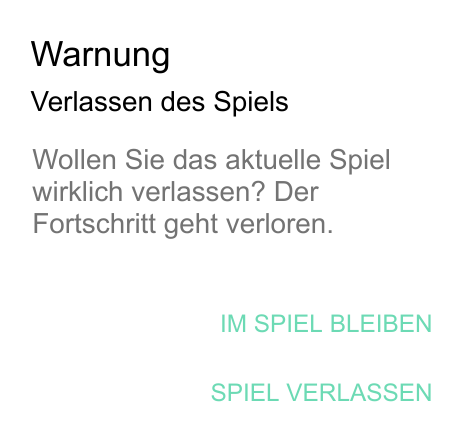
\includegraphics[width=0.4\linewidth]{figures/development/application/abort-message.png}
	}
	\caption{Warnung, die angezeigt wird, wenn der/die Benutzer/in das Spiel vorzeitig verlassen möchte.}
	\label{fig:game-abort-page}
\end{figure}

\paragraph{Shortcuts}
Abkürzungen, die von Anfänger/innen nicht eingesetzt werden, können für Expertenbenutzer/innen einen erheblichen Produktivitätsboost bedeuten. Dadurch ist das System für alle möglichen Benutzer/innengruppen ansprechend. \cite{nielsen:1993:usability}

Ein Beispiel hierfür wären Tastaturshortcuts, die in Textverarbeitungsprogrammen existieren. Die Anwendung erlaubt, dass der Einleitungstext permanent ausgeblendet werden kann (siehe Abbildung \ref{fig:game-introduction-page}). Dazu muss einmalig die Checkbox angeklickt werden. Dies spart erfahrenen Benutzer/innen viel Zeit. Zudem besteht die Möglichkeit diese Einstellung rückgängig zu machen.

\begin{figure}[H]
    \centering
	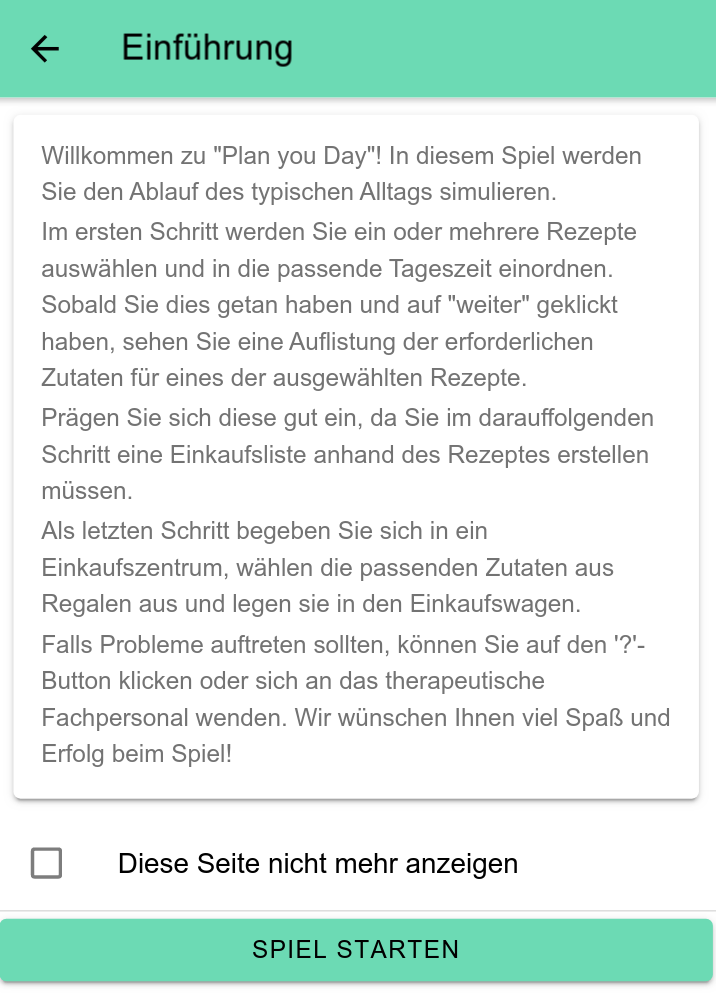
\includegraphics[width=0.4\linewidth]{figures/development/application/introduction.png}
	\caption{Abschnitt mit dem Einführungstext des Spiels.}
	\label{fig:game-introduction-page}
\end{figure}

\paragraph{Good error messages}
Gute Fehlermeldungen sollen in einfacher Sprache verfasst werden und keine systeminternen Bezeichnungen sein. Das vorliegende Problem muss einfach ausgedrückt und eine Lösung vorschlagen werden. \cite{nielsen:1993:usability}

Dem/Der Benutzer/in sollen keine kryptischen Fehlermeldungen angezeigt werden, die direkt vom System ausgegeben werden, sondern verständliche Fehlerbeschreibungen. In der Anwendung wird dem/der Spieler/in klar mitgeteilt, wodurch der Fehler ausgelöst wurde (siehe Abbildung \ref{fig:game-error-message}).

\begin{figure}[H]
    \centering
	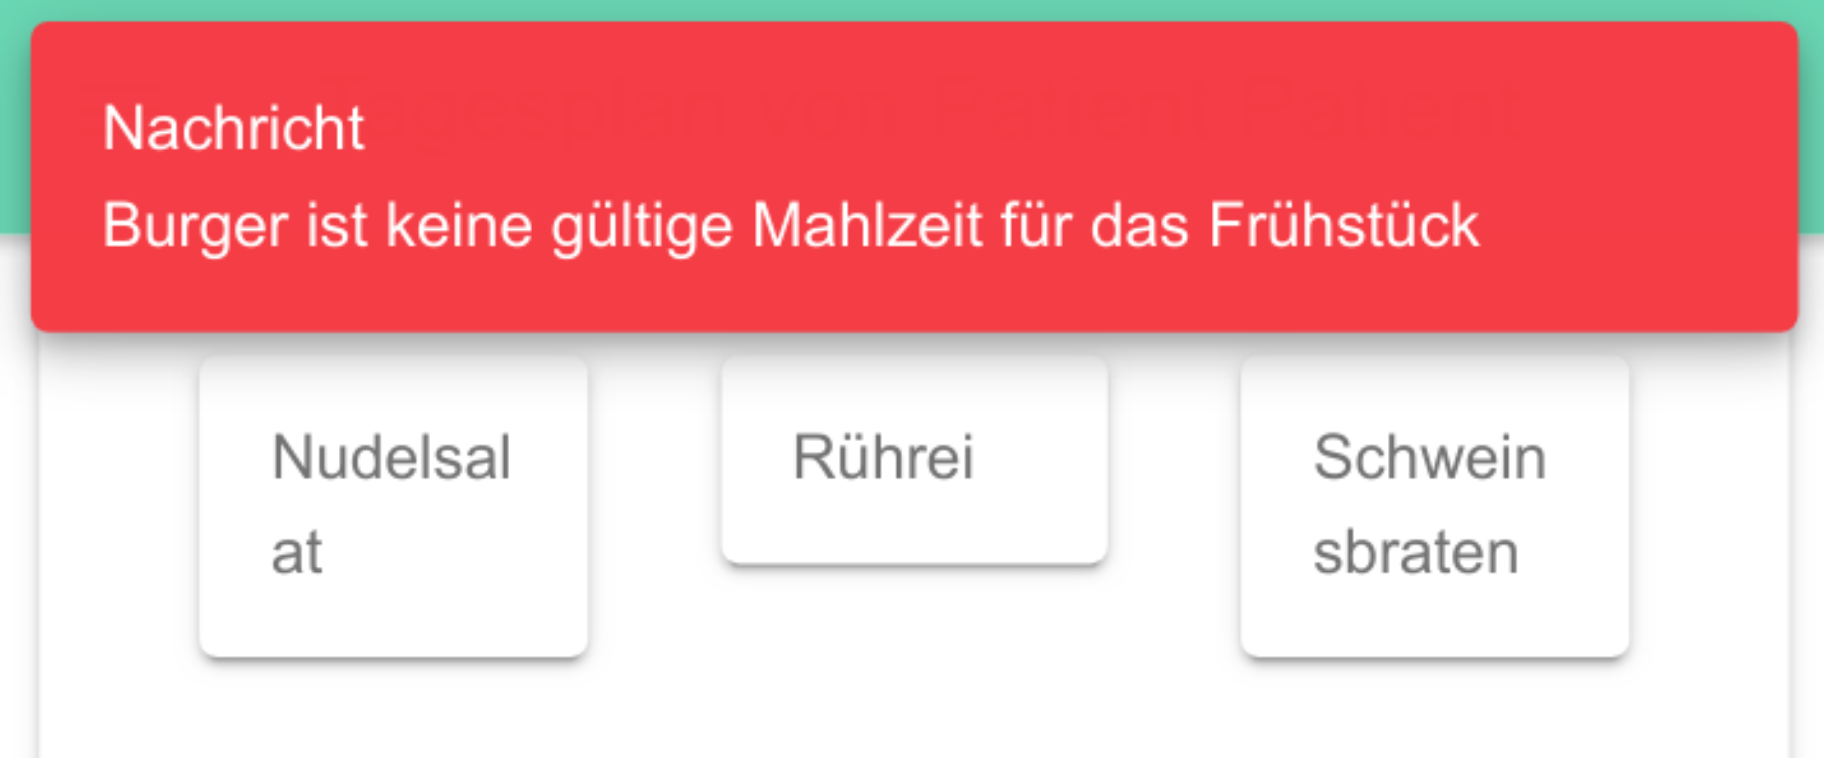
\includegraphics[width=0.5\linewidth]{figures/development/application/error-message.png}
	\caption{Fehlermeldung, die angezeigt wird, wenn der/die Spieler/in eine ungültige Mahlzeit in die Tageszeit \enquote{Frühstück} gezogen hat.}
	\label{fig:game-error-message}
\end{figure}

\paragraph{Prevent errors}
Aussagekräftige Fehlermeldungen sind sehr wichtig, aber noch besser ist, wenn direkt verhindert wird, dass ein Fehler auftritt. Das Design soll es dem/der Benutzer/in erschweren Fehler zu machen. \cite{nielsen:1993:usability}

Dies kann durch den Einsatz einer plattformübergreifenden Designsprache umgesetzt werden. Es existieren einige bekannte Ansätze, etwa das \hyperlink{https://www.microsoft.com/design/fluent/}{Fluent Design} von Microsoft oder das \hyperlink{https://material.io/design/}{Material Design} von Google. Während der Entwicklung wurden die Design-Richtlinien von Google strikt befolgt. 
Laut Google dient das Material Design dazu, dass der verfügbare Platz bestmöglich genutzt wird und ein konsistentes Design auf Smartphones, Tablets und Desktops umgesetzt wird. Das Material Design ist von der physikalischen Welt und deren Texturen inspiriert. Dazu zählt auch wie Licht reflektiert und wie Schatten geworfen werden. \cite{material-design:introduction:2020} \\
Für alle möglichen Komponenten, wie Buttons, Navigationsleisten \acl{usw.}, existieren Best-Practices. Beispielsweise soll eine Top-Bar immer oben sein und dem/der Benutzer/in erlauben, schnell zu navigieren. Der Inhalt darf sich nicht ändern. Dazu existieren noch Empfehlungen in welcher Reihenfolge Symbole in der Leiste angeordnet werden können. Eine Richtlinie ist, dass der Text nicht abgeschnitten werden darf. \cite{material-design:appbar:2020}

\paragraph{Help and documentation}
Am Besten ist, wenn das System ohne Dokumentation verwendbar ist. Trotzdessen sollen Hilfestellungen und Dokumentationen angeboten werden. Diese Informationen müssen einfach zu finden, möglichst kurz und leicht zu verstehen sein. \cite{nielsen:1993:usability}

Der/Die Benutzer/in soll im Falle eines Problems schnell an Hilfe gelangen. In der Anwendung kann der/die User/in in jedem Spielabschnitt den zugehörigen Hilfetext öffnen (siehe Abbildung \ref{fig:game-help-text}). Zudem können alle Zutaten mit Bild außerhalb des Spiels angesehen werden (siehe Abbildung \ref{fig:game-ingredient-info}). Des Weiteren können die Rezepte mit all ihren Bestandteilen, der Schwierigkeit und der Tageszeit angezeigt werden (siehe Abbildung \ref{fig:game-recipe-info}).

\begin{figure}[H]
    \centering
	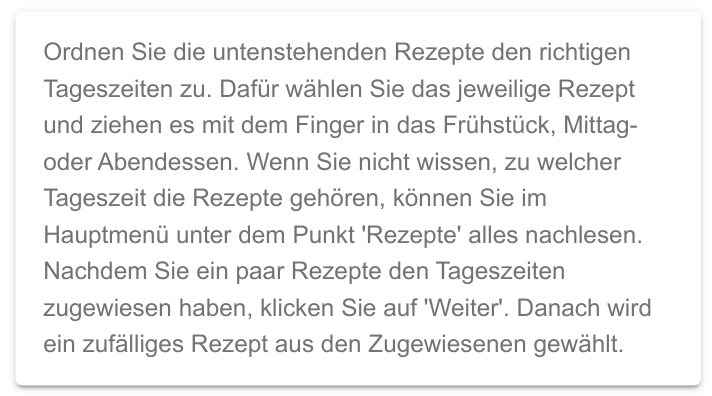
\includegraphics[width=0.5\linewidth]{figures/development/application/helptext.png}
	\caption{Hilfetext des Spielabschnitts \enquote{Tagesplanung}.}
	\label{fig:game-help-text}
\end{figure}

\begin{figure}[H]
    \centering
	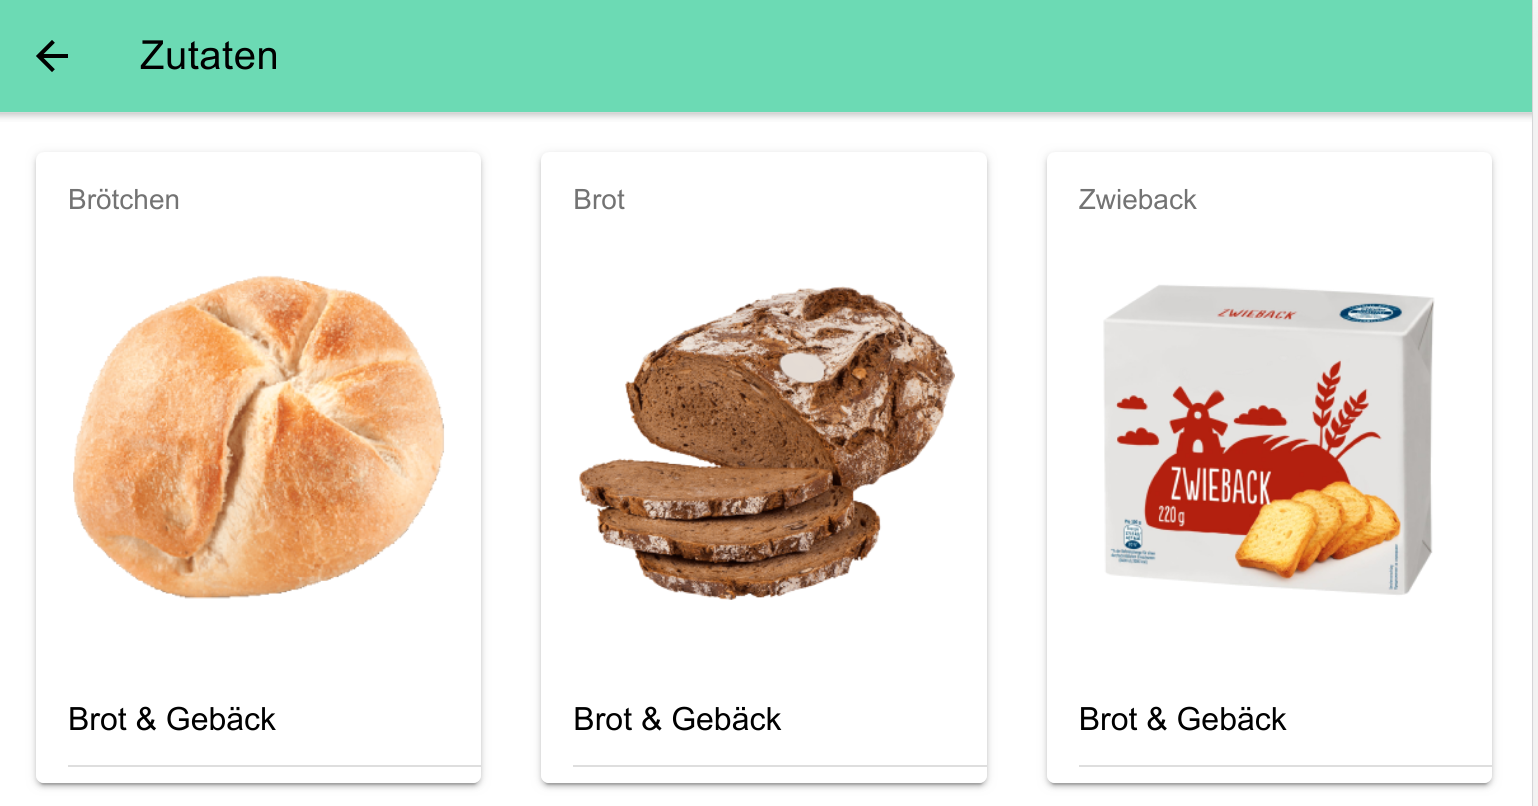
\includegraphics[width=0.5\linewidth]{figures/development/application/ingredient-info.png}
	\caption{Ausschnitt der Überblicksseite über alle Zutaten.}
	\label{fig:game-ingredient-info}
\end{figure}

\begin{figure}[H]
    \centering
	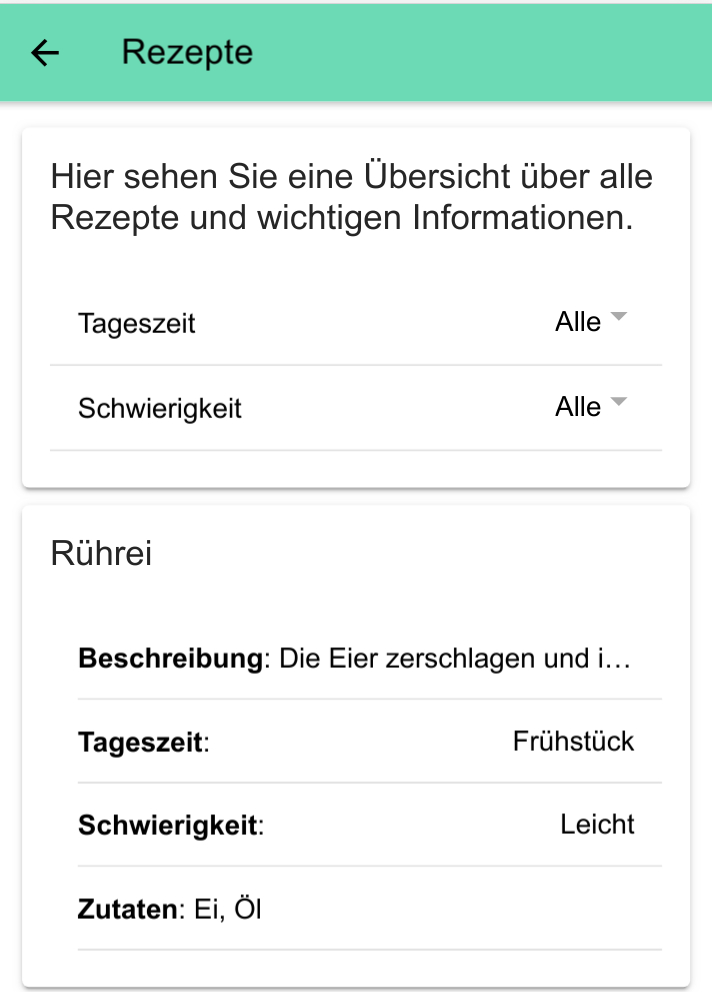
\includegraphics[width=0.35\linewidth]{figures/development/application/recipe-info.png}
	\caption{Ausschnitt der Ansicht, wo alle Rezepte angezeigt werden können. Oben kann zum besseren Überblick nach Tageszeit und Schwierigkeit gefiltert werden.}
	\label{fig:game-recipe-info}
\end{figure}